\iffalse
This file is protected by Copyright. Please refer to the COPYRIGHT file
distributed with this source distribution.

This file is part of OpenCPI <http://www.opencpi.org>

OpenCPI is free software: you can redistribute it and/or modify it under the
terms of the GNU Lesser General Public License as published by the Free Software
Foundation, either version 3 of the License, or (at your option) any later
version.

OpenCPI is distributed in the hope that it will be useful, but WITHOUT ANY
WARRANTY; without even the implied warranty of MERCHANTABILITY or FITNESS FOR A
PARTICULAR PURPOSE. See the GNU Lesser General Public License for more details.

You should have received a copy of the GNU Lesser General Public License along
with this program. If not, see <http://www.gnu.org/licenses/>.
\fi

%----------------------------------------------------------------------------------------
% Update the docTitle and docVersion per document
%----------------------------------------------------------------------------------------
\def\docTitle{Component Data Sheet}
\def\docVersion{1.5}
%----------------------------------------------------------------------------------------
\documentclass{article}
\iffalse
This file is protected by Copyright. Please refer to the COPYRIGHT file
distributed with this source distribution.

This file is part of OpenCPI <http://www.opencpi.org>

OpenCPI is free software: you can redistribute it and/or modify it under the
terms of the GNU Lesser General Public License as published by the Free Software
Foundation, either version 3 of the License, or (at your option) any later
version.

OpenCPI is distributed in the hope that it will be useful, but WITHOUT ANY
WARRANTY; without even the implied warranty of MERCHANTABILITY or FITNESS FOR A
PARTICULAR PURPOSE. See the GNU Lesser General Public License for more details.

You should have received a copy of the GNU Lesser General Public License along
with this program. If not, see <http://www.gnu.org/licenses/>.
\fi
\author{} % Force author to be blank
%----------------------------------------------------------------------------------------
% Paper size, orientation and margins
%----------------------------------------------------------------------------------------
\usepackage{geometry}
\geometry{
        letterpaper, % paper type
        portrait,    % text direction
        left=.75in,  % left margin
        top=.75in,   % top margin
        right=.75in, % right margin
        bottom=.75in % bottom margin
 }
%----------------------------------------------------------------------------------------
% Header/Footer
%----------------------------------------------------------------------------------------
\usepackage{fancyhdr} \pagestyle{fancy} % required for fancy headers
\renewcommand{\headrulewidth}{0.5pt}
\renewcommand{\footrulewidth}{0.5pt}
\rhead{\small{ANGRYVIPER Team}}
% \rfoot{\thepage}
%----------------------------------------------------------------------------------------
% Appendix packages
%----------------------------------------------------------------------------------------
\usepackage[toc,page]{appendix}
%----------------------------------------------------------------------------------------
% Defined Commands & Renamed Commands
%----------------------------------------------------------------------------------------
\renewcommand{\contentsname}{Table of Contents}
\renewcommand{\listfigurename}{List of Figures}
\renewcommand{\listtablename}{List of Tables}
%----------------------------------------------------------------------------------------
% Various packages
%----------------------------------------------------------------------------------------
\usepackage[usenames,dvipsnames]{xcolor} % for color names see https://en.wikibooks.org/wiki/LaTeX/Colors
\usepackage{hyperref}  % for linking urls and lists
\usepackage{graphicx}  % for including pictures by file
\usepackage{listings}  % for coding language styles
\usepackage{rotating}  % for sideways table
\usepackage{pifont}    % for sideways table
\usepackage{pdflscape} % for landscape view
\usepackage{subfig}
\usepackage{xstring}
\uchyph=0 % Never hyphenate acronyms like RCC (I think this overrides ANGRYVIPER above)
\renewcommand\_{\textunderscore\allowbreak} % Allow words to break/newline on underscores
%----------------------------------------------------------------------------------------
% Table packages
%----------------------------------------------------------------------------------------
\usepackage{longtable} % for long possibly multi-page tables
\usepackage{tabularx} % c=center,l=left,r=right,X=fill
% These define tabularx columns "C" and "R" to match "X" but center/right aligned
\newcolumntype{C}{>{\centering\arraybackslash}X}
\newcolumntype{R}{>{\raggedleft\arraybackslash}X}
\usepackage{float}
\floatstyle{plaintop}
\usepackage[tableposition=top]{caption}
\newcolumntype{P}[1]{>{\centering\arraybackslash}p{#1}}
\newcolumntype{M}[1]{>{\centering\arraybackslash}m{#1}}
%----------------------------------------------------------------------------------------
% Block Diagram / FSM Drawings
%----------------------------------------------------------------------------------------
\usepackage{tikz}
\usetikzlibrary{shapes,arrows,fit,positioning}
\usetikzlibrary{automata} % used for the fsm
%----------------------------------------------------------------------------------------
% Colors Used
%----------------------------------------------------------------------------------------
\usepackage{colortbl}
\definecolor{blue}{rgb}{.7,.8,.9}
\definecolor{ceruleanblue}{rgb}{0.16, 0.32, 0.75}
\definecolor{drkgreen}{rgb}{0,0.6,0}
\definecolor{deepmagenta}{rgb}{0.8, 0.0, 0.8}
\definecolor{cyan}{rgb}{0.0,0.6,0.6}
\definecolor{maroon}{rgb}{0.5,0,0}
%----------------------------------------------------------------------------------------
% VHDL Coding Language Style
% modified from: http://latex-community.org/forum/viewtopic.php?f=44&t=22076
%----------------------------------------------------------------------------------------
\lstdefinelanguage{VHDL}
{
        basicstyle=\ttfamily\footnotesize,
        columns=fullflexible,keepspaces,      % https://tex.stackexchange.com/a/46695/87531
        keywordstyle=\color{ceruleanblue},
        commentstyle=\color{drkgreen},
        morekeywords={
    library,use,all,entity,is,port,in,out,end,architecture,of,
    begin,and, signal, when, if, else, process, end,
        },
        morecomment=[l]--
}
%----------------------------------------------------------------------------------------
% XML Coding Language Style
% modified from: http://tex.stackexchange.com/questions/10255/xml-syntax-highlighting
%----------------------------------------------------------------------------------------
\lstdefinelanguage{XML}
{
        basicstyle=\ttfamily\footnotesize,
        columns=fullflexible,keepspaces,
        morestring=[s]{"}{"},
        morecomment=[s]{!--}{--},
        commentstyle=\color{drkgreen},
        moredelim=[s][\color{black}]{>}{<},
        moredelim=[s][\color{cyan}]{\ }{=},
        stringstyle=\color{maroon},
        identifierstyle=\color{ceruleanblue}
}
%----------------------------------------------------------------------------------------
% DIFF Coding Language Style
% modified from http://tex.stackexchange.com/questions/50176/highlighting-a-diff-file
%----------------------------------------------------------------------------------------
\lstdefinelanguage{diff}
{
        basicstyle=\ttfamily\footnotesize,
        columns=fullflexible,keepspaces,
        breaklines=true,                                % wrap text
        morecomment=[f][\color{ceruleanblue}]{@@},      % group identifier
        morecomment=[f][\color{red}]-,                  % deleted lines
        morecomment=[f][\color{drkgreen}]+,             % added lines
        morecomment=[f][\color{deepmagenta}]{---},      % Diff header lines (must appear after +,-)
        morecomment=[f][\color{deepmagenta}]{+++},
}
%----------------------------------------------------------------------------------------
% Python Coding Language Style
% modified from
%----------------------------------------------------------------------------------------
\lstdefinelanguage{python}
{
        basicstyle=\ttfamily\footnotesize,
        columns=fullflexible,keepspaces,
        keywordstyle=\color{ceruleanblue},
        commentstyle=\color{drkgreen},
        stringstyle=\color{orange},
        morekeywords={
    print, if, sys, len, from, import, as, open,close, def, main, for, else, write, read, range,
        },
        comment=[l]{\#}
}
%----------------------------------------------------------------------------------------
% Fontsize Notes in order from smallest to largest
%----------------------------------------------------------------------------------------
%    \tiny
%    \scriptsize
%    \footnotesize
%    \small
%    \normalsize
%    \large
%    \Large
%    \LARGE
%    \huge
%    \Huge

\date{Version \docVersion} % Force date to be blank and override date with version
\title{\docTitle}
\lhead{\small{\docTitle}}

\usepackage{longtable} % for long possibly multi-page tables

\def\comp{iqstream\_to\_timeiq}
\def\ecomp{iqstream_to_timeiq}
\def\Comp{IQstream to TimeIQ}
\graphicspath{ {figures/} }

\begin{document}

\section*{Summary - \Comp}
\begin{tabular}{|c|M{13.5cm}|}
	\hline
	\rowcolor{blue}
	                  &                        							\\
	\hline
	Name              & \comp                  							\\
	\hline
	Worker Type       & Application            							\\
	\hline
	Version           & \docVersion                  							\\
	\hline
	Release Date      & 4/2019           						\\
	\hline
	Component Library & ocpi.assets.misc\_comps 					\\
	\hline
	Workers           & \comp.hdl              							\\
	\hline
	Tested Platforms  & isim, xsim, modelsim, zed, matchstiq\_z1, e3xx, alst4, ml605	\\
	\hline
\end{tabular}
	
\section*{Functionality}
\begin{flushleft}
	The \Comp{} component adapts the iqstream protocol to the TimeStamped\_IQ protocol.
\end{flushleft}

\section*{Worker Implementation Details}
\subsection*{\comp.hdl}
\begin{flushleft}
	The TimeStamped\_IQ protocol consists of multiple opcodes which include complex IQ samples, and the iqstream protocol consists only of complex IQ samples. The \comp{} worker forwards data from the input port to the output port and applies the samples opcode to it.
\end{flushleft}

\section*{Block Diagrams}
\subsection*{Top level}
\begin{center}
	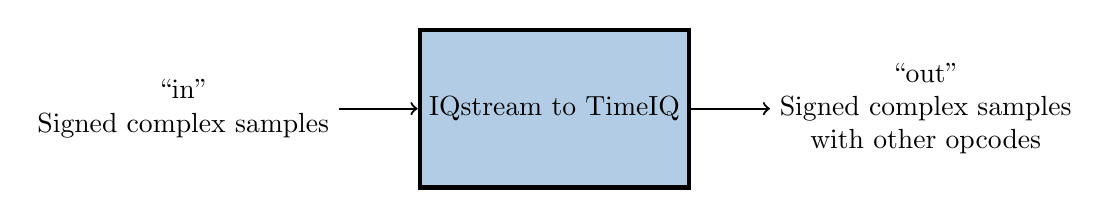
\begin{tikzpicture}[% List of styles applied to all, to override specify on a case-by-case
			every node/.style={	
				align=center,  		% use this so that the "\\" for line break works
				minimum size=2cm	% creates space above and below text in rectangle
			},
			every edge/.style={draw,thick}
		]
		\node[rectangle,ultra thick,draw=black,fill=blue](R2){\Comp};
		\node[rectangle,draw=white,fill=white](R3)[left= of R2]{``in" \\ Signed complex samples};
		\node[rectangle,draw=white,fill=white](R4)[right= of R2]{``out" \\ Signed complex samples\\ with other opcodes};
		\path[->]
		(R3)edge []	node [] {} (R2)
		(R2)edge []	node [] {} (R4)
		;
	\end{tikzpicture}
\end{center}

\section*{Source Dependencies}
\subsection*{\comp.hdl}
\begin{itemize}
	\item bsp\_picoflexor/components/\comp.hdl/\comp.vhd
\end{itemize}

\begin{landscape}
	\section*{Component Spec Properties}
	There are no component spec properties for this component
	
	\section*{Worker Properties}
	There are no worker implementation-specific properties for this component
	
	\section*{Component Ports}
	\begin{scriptsize}
		\begin{tabular}{|M{2cm}|M{1.5cm}|M{4cm}|c|c|M{9cm}|}
			\hline
			\rowcolor{blue}
			Name & Producer & Protocol                       & Optional & Advanced & Usage                                  		\\
			\hline
			in   & false    & iqstream\_protocol			 & false    & -        & Signed complex samples 						\\
			\hline
			out  & true     & TimeStamped\_IQ-prot           & false    & -        & Signed complex samples plus other operations   \\
			\hline
		\end{tabular}
	\end{scriptsize}
	\section*{Worker Interfaces}
	\subsection*{\comp.hdl}
	\begin{scriptsize}
		\begin{tabular}{|M{2cm}|M{1.5cm}|c|c|M{12cm}|}
			\hline
			\rowcolor{blue}
			Type            & Name & DataWidth & Advanced   & Usage                                    		\\
			\hline
			StreamInterface & in   & 32        & - 			& Signed complex samples 						\\
			\hline
			StreamInterface & out  & 32        & - 			& Signed complex samples plus other operations	\\
			\hline
		\end{tabular}
	\end{scriptsize}
\end{landscape}

\section*{Control Timing and Signals}
\begin{flushleft}
	The \comp worker{} uses the clock from the Control Plane and standard Control Plane signals.\\
\end{flushleft}

\begin{landscape}
\section*{Worker Configuration Parameters}
\subsubsection*{\comp.hdl}
\input{../../\ecomp.hdl/configurations.inc}
\section*{Performance and Resource Utilization}
\input{../../\ecomp.hdl/utilization.inc}
\end{landscape}

\section*{Test and Verification}
\begin{flushleft}
	The input file contains 5824 bytes of arbitrary data. It is the same input file used for the TimeIQ\_to\_IQstream unit test. The expected output waveform is identical to the input file.
\end{flushleft}
\end{document}
